% Week 3 Engineering Progress Deck — ISSCC/VLSI Minimalist Theme (20 Pages, Pure English)
% Build: python3 make_data.py && latexmk -xelatex main.tex
% All metric values are generated into data/ from verified repository records; none are hardcoded here.
\documentclass[10pt,aspectratio=169,hyperref={colorlinks,urlcolor=steel,linkcolor=}]{beamer}
\usepackage{PekingU}
\setbeamertemplate{headline}{}
\makeatletter\AtBeginDocument{\global\pku@headheight=0pt}\makeatother
\setbeamertemplate{background canvas}{\color{white}\rule{\paperwidth}{\paperheight}}
\usefonttheme{professionalfonts}
\usepackage{fontspec}
\usepackage{xeCJK}
\xeCJKsetup{CJKmath=true}
% CJK: Microsoft YaHei (TrueType collection) on Windows/WSL; PingFang SC on macOS; Noto Sans CJK SC on Linux. Never the ctex default serif.
\IfFileExists{/mnt/c/Windows/Fonts/msyh.ttc}{%
  \setCJKmainfont{msyh.ttc}[Path=/mnt/c/Windows/Fonts/,BoldFont=msyhbd.ttc,ItalicFont=msyh.ttc]%
  \setCJKsansfont{msyh.ttc}[Path=/mnt/c/Windows/Fonts/,BoldFont=msyhbd.ttc,ItalicFont=msyh.ttc]%
  \setCJKmonofont{msyh.ttc}[Path=/mnt/c/Windows/Fonts/,BoldFont=msyhbd.ttc,ItalicFont=msyh.ttc]%
}{%
  \IfFontExistsTF{PingFang SC}{%
    \setCJKmainfont{PingFang SC}\setCJKsansfont{PingFang SC}\setCJKmonofont{PingFang SC}%
  }{%
    \setCJKmainfont{Noto Sans CJK SC}\setCJKsansfont{Noto Sans CJK SC}\setCJKmonofont{Noto Sans CJK SC}%
  }%
}
\renewcommand{\CJKfamilydefault}{\CJKsfdefault}

% Strictly TrueType (.ttf) sans-serif & monospace fonts for universal pdf.js rendering
\IfFileExists{/mnt/c/Windows/Fonts/segoeui.ttf}{%
  \setsansfont{segoeui.ttf}[
    Path=/mnt/c/Windows/Fonts/,
    BoldFont=segoeuib.ttf,
    ItalicFont=segoeuii.ttf,
    BoldItalicFont=segoeuiz.ttf
  ]%
}{%
  \IfFontExistsTF{Helvetica Neue}{%
    \setsansfont{Helvetica Neue}%
  }{%
    \setsansfont{LiberationSans-Regular.ttf}[
      Path=/usr/share/fonts/truetype/liberation/,
      BoldFont=LiberationSans-Bold.ttf,
      ItalicFont=LiberationSans-Italic.ttf,
      BoldItalicFont=LiberationSans-BoldItalic.ttf
    ]%
  }%
}
\IfFileExists{/mnt/c/Windows/Fonts/consola.ttf}{%
  \setmonofont{consola.ttf}[
    Path=/mnt/c/Windows/Fonts/,
    BoldFont=consolab.ttf,
    Scale=0.92
  ]%
}{%
  \IfFontExistsTF{Menlo}{%
    \setmonofont{Menlo}[Scale=0.92]%
  }{%
    \setmonofont{LiberationMono-Regular.ttf}[
      Path=/usr/share/fonts/truetype/liberation/,
      BoldFont=LiberationMono-Bold.ttf,
      Scale=0.92
    ]%
  }%
}
\renewcommand{\familydefault}{\sfdefault}

\usepackage{amsmath,amssymb,xcolor,booktabs,graphicx,ragged2e,parskip,tabularx,array,multirow,colortbl}
\usepackage{tikz}
\usetikzlibrary{positioning,arrows.meta,calc}
\usepackage{pgfplots}
\pgfplotsset{compat=1.18}
\apptocmd{\frame}{}{\justifying}{}

\input{data/numbers.tex}
\makeatletter\newcommand{\tabinput}[1]{\@@input #1 }\makeatother

% ---------- ISSCC / VLSI Restrained Minimalist Palette ----------
\definecolor{peking}{HTML}{8B0012}     % Primary Accent: PKU Crimson
\definecolor{ink}{HTML}{1E293B}        % Primary Ink: Deep Charcoal
\definecolor{muted}{HTML}{64748B}      % Secondary Text / Captions
\definecolor{hair}{HTML}{D8DEE6}       % Hairline Rules & Borders
\definecolor{surf}{HTML}{F6F7F9}       % Neutral Light Surface
\definecolor{steel}{HTML}{1D4E89}      % Secondary Chart Accent: Deep Steel Blue
\definecolor{passink}{HTML}{15803D}    % Subtle Semantic Pass
\definecolor{warnink}{HTML}{B45309}    % Subtle Semantic Attention

\setbeamercolor{normal text}{fg=ink,bg=white}
\setbeamercolor{frametitle}{fg=peking,bg=white}
\setbeamercolor{structure}{fg=peking}
\setbeamercolor{footline}{bg=peking,fg=white}
\setbeamercolor{title}{bg=peking,fg=white}
\setbeamerfont{frametitle}{series=\bfseries,size=\large}
\setbeamerfont{section in toc}{series=\bfseries,size=\normalsize}
\setbeamerfont{itemize/enumerate body}{size=\scriptsize}
\setbeamerfont{itemize/enumerate subbody}{size=\scriptsize}
\setbeamertemplate{itemize item}{\raisebox{0.18ex}{\tikz\fill[peking] (0,0) rectangle (3pt,3pt);}}
\setbeamertemplate{itemize subitem}{\raisebox{0.18ex}{\tikz\draw[muted,line width=0.6pt] (0,0) circle (1.3pt);}}
\setbeamertemplate{enumerate item}{\textbf{\color{peking}\insertenumlabel.}}

\title[先进芯片全栈设计与实践]{先进芯片全栈设计与实践\\[3pt]{\large Full-Stack Chip Design \& Practice}}
\subtitle{第 3 周进展：从架构与 RTL 到物理签核（Signoff）与主机加速}
\author[]{Ruijun He \quad Guoyi Zhang \quad Zhiyuan Zhao \quad Muyang Cheng}
\institute{Peking University}
\date{November 2026}

% ---------- Clean Helpers ----------
\newcommand{\hl}[1]{\textcolor{peking}{\textbf{#1}}}
\newcommand{\snote}[1]{{\scriptsize\color{muted}#1\par}}
\newcommand{\ok}{\tikz[baseline=-0.1ex]\draw[passink,line width=1.15pt,line cap=round,line join=round] (0,0.34ex) -- (0.36ex,-0.02ex) -- (0.98ex,0.82ex);}
\newcommand{\pending}{\textcolor{warnink}{\textbf{–}}}
\newcommand{\abi}{ABI 5.0 \NCols×\NCols}

% Crisp Left-Bar Callout (Zero full-sided colored boxes)
\newcommand{\callout}[2][peking]{%
  \noindent\begin{tikzpicture}
    \node[anchor=north west, fill=surf, text=ink, inner xsep=8pt, inner ysep=6pt,
          text width=\dimexpr\linewidth-16pt\relax, align=left, font=\scriptsize] (box) {#2};
    \fill[#1] (box.north west) rectangle ([xshift=2.4pt]box.south west);
  \end{tikzpicture}%
}

\tikzset{
  issccbox/.style={draw=ink!80, line width=0.75pt, rounded corners=1.5pt, fill=white,
                   align=center, font=\scriptsize, inner sep=4pt, minimum height=0.95cm, text width=#1},
  issccbox/.default=1.8cm,
  issccarr/.style={-{Stealth[length=4.5pt,width=3.2pt]}, line width=0.75pt, draw=ink!80},
  issccnote/.style={font=\tiny, text=ink!85, inner sep=1pt, outer sep=2pt},
}

\pgfplotsset{
  issccbar/.style={
    font=\scriptsize,
    axis lines*=left,
    axis line style={ink!60, line width=0.6pt},
    tick style={ink!50},
    grid style={hair, line width=0.4pt},
    tick label style={font=\scriptsize, text=ink},
    xticklabel={\pgfmathprintnumber[assume math mode=true]{\tick}},
    yticklabel={\pgfmathprintnumber[assume math mode=true]{\tick}},
    label style={font=\scriptsize, text=ink},
    legend style={font=\scriptsize, draw=none, fill=none},
    /pgf/number format/assume math mode=true,
  },
}

\setlength{\tabcolsep}{4pt}
\renewcommand{\arraystretch}{1.18}

% Clean Minimalist Chapter Divider Slides
\AtBeginSection[]{}

\begin{document}

% ===================================================================== 1 Cover
{\setbeamertemplate{logo}{}
\begin{frame}
  \titlepage
  \begin{center}
\includegraphics[width=0.21\linewidth]{Figures/PKU-emblem-names.png}\end{center}
\end{frame}}

% ===================================================================== 2 Overview
\begin{frame}{总览：第 3 周端到端进展}
  \begin{columns}[T,onlytextwidth]
    \column{0.238\textwidth}
      {\color{ink}\rule{\linewidth}{1.6pt}}\par\vspace{5pt}
      {\tiny\bfseries\color{muted} 01 · 架构与 RTL}\\[2pt]
      {\small\bfseries\color{ink} SRAM 化 Lookup}\\[5pt]
      {\large\bfseries\color{peking} \NLookupAreaPct\%} {\scriptsize\color{muted} 查找表面积}\\[4pt]
      \begin{itemize}\setlength{\itemsep}{2pt}
        \item \NLookupFFBefore{} → \NLookupFFAfter{} 个 FF
        \item \NRtlModels{} 模型 × \NRtlConfigs{} 配置 \NRtlExactShort
        \item Lookup mutant 杀死 \NMutKilled/\NMutNew
      \end{itemize}
    \column{0.238\textwidth}
      {\color{peking}\rule{\linewidth}{1.6pt}}\par\vspace{5pt}
      {\tiny\bfseries\color{peking} 02 · 统一 ASIC 签核}\\[2pt]
      {\small\bfseries\color{ink} Single-GDS 流程}\\[5pt]
      {\large\bfseries\color{peking} \NSealSide\,µm} {\scriptsize\color{muted} 封环管芯}\\[4pt]
      \begin{itemize}\setlength{\itemsep}{2pt}
        \item TT \NCoreMHz{} MHz, \NMmmcCorners-Corner MMMC
        \item DRC / nmLVS / ANT / WireBond \NSignoffAllStatus
        \item ERC \NErcHier{} Hier. / \NErcExp{} Exp. 已逐项审计
      \end{itemize}
    \column{0.238\textwidth}
      {\color{ink}\rule{\linewidth}{1.6pt}}\par\vspace{5pt}
      {\tiny\bfseries\color{muted} 03 · 主机与 FPGA}\\[2pt]
      {\small\bfseries\color{ink} Single-RPC 流水线}\\[5pt]
      {\large\bfseries\color{peking} \NRpcBatchedMax{} → \NRpcPipe} {\scriptsize\color{muted} 主机 RPC 次数}\\[4pt]
      \begin{itemize}\setlength{\itemsep}{2pt}
        \item RPC 实测减少 \NRpcSpMin–\NRpcSpMax×
        \item \NRtlTckMhz{} MHz RTL + \NRpcExactCount/\NRpcModels{} TclRpc golden-output fixture \NRpcExactStatus
      \end{itemize}
    \column{0.238\textwidth}
      {\color{ink}\rule{\linewidth}{1.6pt}}\par\vspace{5pt}
      {\tiny\bfseries\color{muted} 04 · 应用}\\[2pt]
      {\small\bfseries\color{ink} 六场景套件}\\[5pt]
      {\large\bfseries\color{peking} \NDemoGolden/\NDemoGoldenTotal} {\scriptsize\color{muted} INT32 \NDemoExactStatus}\\[4pt]
      \begin{itemize}\setlength{\itemsep}{2pt}
        \item \NDemoZoo/\NDemoZoo{} zoo 参考帧 \NDemoExactStatus
        \item \NDemoFixes{} 项运行时健壮性修复
      \end{itemize}
  \end{columns}\par\vspace{12pt}\callout[peking]{\textbf{核心主线}：以 SRAM 化 Lookup 释放面积（\hl{\NLookupAreaPct\%}），在统一 \texttt{postDummy.gds} 上完成 DRC / nmLVS / ANT / WireBond 签核与 ERC 审计，再以 Single-RPC 把主机 RPC 由 \NRpcBatchedMax{} 次压至 \NRpcPipe{} 次；Phase B 转向真 MMMC 与实板 USB 批量后端。}
\end{frame}

% ##################################################################### PART 01
\section{架构与 RTL 验证}

\begin{frame}{\texttt{npu\_tensor\_lookup}：从触发器迁移到 Activation SRAM}
  \begin{columns}[T,onlytextwidth]
    \column{0.40\textwidth}
    \textbf{设计动机}
    \begin{itemize}\setlength{\itemsep}{2pt}
      \item Lookup 溯源记录仅在 \texttt{MODEL\_COMMIT} 阶段查询，用于校验每个源张量均已写入且未被覆盖。
      \item commit 期间 Activation SRAM 不存放有效激活值，并在推理 \texttt{START} 前清空。
    \end{itemize}\par\vspace{5pt}
    \textbf{实现方案}
    \begin{itemize}\setlength{\itemsep}{2pt}
      \item 以顺序 SRAM 扫描替换 \NRecords×\NRecordBitsOld-bit 的 FF 表（占优化前 stdcell 面积的 \NLookupShareBefore\%）。
      \item 每条记录打包为 1 个 \NRecordWordBits-bit 字，存放于 Activation SRAM 字节区间 \texttt{[0, 4(op+1))}。
      \item 复用现有 SRAM 读写端口，顶层 SRAM 引脚零新增。
    \end{itemize}\par\vspace{7pt}
    \callout[peking]{\textbf{综合实测收益}：Lookup FF \NLookupFFBefore{} → \hl{\NLookupFFAfter}；模块面积 \NLookupAreaBefore{} → \hl{\NLookupAreaAfter{} kµm²}（\hl{\NLookupAreaPct\%}）。}
    \column{0.57\textwidth}
    \centering
    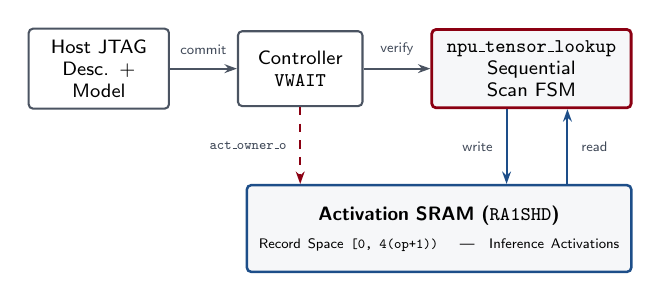
\begin{tikzpicture}[node distance=0.55cm and 0.85cm]
      \node[issccbox=1.5cm] (host) {Host JTAG\\Desc. + Model};
      \node[issccbox=1.3cm, right=of host] (ctl) {Controller\\\texttt{VWAIT}};
      \node[issccbox=2.25cm, right=of ctl, fill=surf, draw=peking, line width=1.0pt] (lk) {\textbf{\texttt{npu\_tensor\_lookup}}\\Sequential Scan FSM};
      \node[issccbox=4.6cm, below=0.95cm of lk.south east, anchor=north east, fill=surf, draw=steel, line width=0.9pt, minimum height=1.1cm] (sram) {%
        \textbf{Activation SRAM (\texttt{RA1SHD})}\\[2pt]
        \tiny Record Space \texttt{[0, 4(op+1))} \quad|\quad Inference Activations};
      \draw[issccarr] (host) -- node[issccnote, above=2pt]{commit} (ctl);
      \draw[issccarr] (ctl) -- node[issccnote, above=2pt]{verify} (lk);
      \draw[issccarr, steel] ([xshift=-9pt]lk.south) -- node[issccnote, left=2pt]{write} ([xshift=-9pt]lk.south |- sram.north);
      \draw[issccarr, steel] ([xshift=13pt]lk.south |- sram.north) -- node[issccnote, right=2pt]{read} ([xshift=13pt]lk.south);
      \draw[issccarr, dashed, peking] (ctl.south) -- node[issccnote, left=2pt]{\texttt{act\_owner\_o}} (ctl.south |- sram.north);
    \end{tikzpicture}\par\vspace{10pt}
    {\scriptsize
    \begin{tabular}{@{}l l@{}}
      \toprule
      \textbf{序关系不变量} & \textbf{防护的冒险} \\ \midrule
      同一时刻至多 1 个 SRAM 写在途 & 写后读（RAW）冒险 \\
      写停顿期间不发起读 & 读到过期溯源记录 \\
      \texttt{done} 等待最后一次写被接受 & 主机输入覆写与记录写入冲突 \\
      \texttt{VWAIT} 内锁定端口所有权 & 校验扫描被饿死 \\ \bottomrule
    \end{tabular}}
  \end{columns}
\end{frame}

\begin{frame}{同基线 RTL 回归与 Mutation 覆盖}
  \begin{columns}[T,onlytextwidth]
    \column{0.53\textwidth}
    \textbf{\NRtlModels{} 个 zoo 模型冷运行周期变化量}\par\vspace{3pt}
    {\scriptsize\setlength{\tabcolsep}{3pt}
    \begin{tabular}{@{}lrrrr@{}}
      \toprule
      \textbf{模型} & \textbf{行为级} & \textbf{Δ} & \textbf{\texttt{FPGA\_MEM}} & \textbf{Δ\%} \\ \midrule
      \tabinput{data/cycle_rows.tex}
      \bottomrule
    \end{tabular}}\par\vspace{5pt}
    \snote{\NRtlRuns{} 次对比运行\NRtlExactStatus；\NCycDeltaMin–\NCycDeltaMax{} 周期收益来自 \texttt{START} 时跳过 commit 重扫。\NRtlNeg{} 条负向生命周期检查\NRtlNegStatus。}
    \column{0.44\textwidth}
    \textbf{完整回归门控}\par\vspace{3pt}
    {\scriptsize
    \begin{tabular}{@{}lr@{}}
      \toprule
      行为级程序回归 & \NRegBeh \\
      \texttt{FPGA\_MEM} 程序回归 & \NRegFpga \\
      \texttt{RA1SHD} 宏单元仿真 & \NRegMacro \\
      CDC 边界模糊/扫描 & \NCdcLimits \\
      基线严格 Mutation 套件 & \NMutOld \\ \bottomrule
    \end{tabular}}\par\vspace{7pt}
    \textbf{新 Lookup Mutant：\hl{\NMutKilled/\NMutNew{} 已杀灭（\NMutKillPct\%）}}\par\vspace{3pt}
    {\tiny\setlength{\tabcolsep}{2.5pt}
    \begin{tabular}{@{}lll@{}}
      \toprule
      \textbf{ID} & \textbf{范围} & \textbf{注入故障} \\ \midrule
      \tabinput{data/mutants.tex}
      \bottomrule
    \end{tabular}}
  \end{columns}
\end{frame}

% ##################################################################### PART 02
\section{统一 ASIC 实现与物理签核}

\begin{frame}{综合与布线后相对 FF-Lookup 基线的变化}
  \begin{columns}[T,onlytextwidth]
    \column{0.44\textwidth}
    \centering
    \begin{tikzpicture}
      \begin{axis}[issccbar, xbar, width=0.95\linewidth, height=5.1cm, bar width=8pt, bar shift=0pt,
          xmin=0, xmax=122, xlabel={相对 FF-Lookup 基线降幅（\%）},
          symbolic y coords/.expand once=\NDeltaTicks, ytick/.expand once=\NDeltaTicks, y dir=reverse,
          nodes near coords={−\pgfmathprintnumber[fixed,precision=2]{\pgfplotspointmeta}\%},
          nodes near coords style={font=\tiny, text=ink}, xmajorgrids, enlarge y limits=0.12]
        \input{data/delta_plot.tex}
      \end{axis}
    \end{tikzpicture}\par\vspace{3pt}
    \snote{Single-GDS 签核流程：对角双 SRAM 平面规划，目标利用率 \NUtilPct\%，Hold 目标 \NHoldTarget{} ns。}
    \column{0.53\textwidth}
    {\scriptsize\setlength{\tabcolsep}{3.5pt}
    \begin{tabular}{@{}lrr@{}}
      \toprule
      \textbf{指标} & \textbf{FF 基线} & \textbf{SRAM Lookup} \\ \midrule
      \texttt{npu\_tensor\_lookup} FF & \NLookupFFBefore & \hl{\NLookupFFAfter} \\
      Lookup 模块面积（kµm²） & \NLookupAreaBefore & \hl{\NLookupAreaAfter} \\
      综合 stdcell 面积（mm²） & \NSynStdBefore & \NSynStdAfter \\
      综合时序单元数 & \NSynSeqBefore & \NSynSeqAfter \\
      布线后有效 stdcell（mm²） & \NActBefore & \NActAfter \\
      布线线长（m） & \NWireBefore & \NWireAfter \\
      无向量 TT 功耗（mW） & \NVlessBefore & \NVlessAfter \\ \bottomrule
    \end{tabular}}\par\vspace{7pt}
    \textbf{布线后层次面积分解（kµm²）}\par\vspace{2pt}
    {\scriptsize\setlength{\tabcolsep}{2.5pt}
    \begin{tabular}{@{}lrrrr@{}}
      \toprule
      \textbf{层次} & \textbf{优化前} & \textbf{优化后} & \textbf{Δ} & \textbf{时序单元} \\ \midrule
      \tabinput{data/hier_rows.tex}
      \bottomrule
    \end{tabular}}
  \end{columns}
\end{frame}

\begin{frame}{物理版图、\NPadCount-Pad Keepout 与功能闭合}
  \centering
  \begin{tabular}{@{}cccc@{}}
    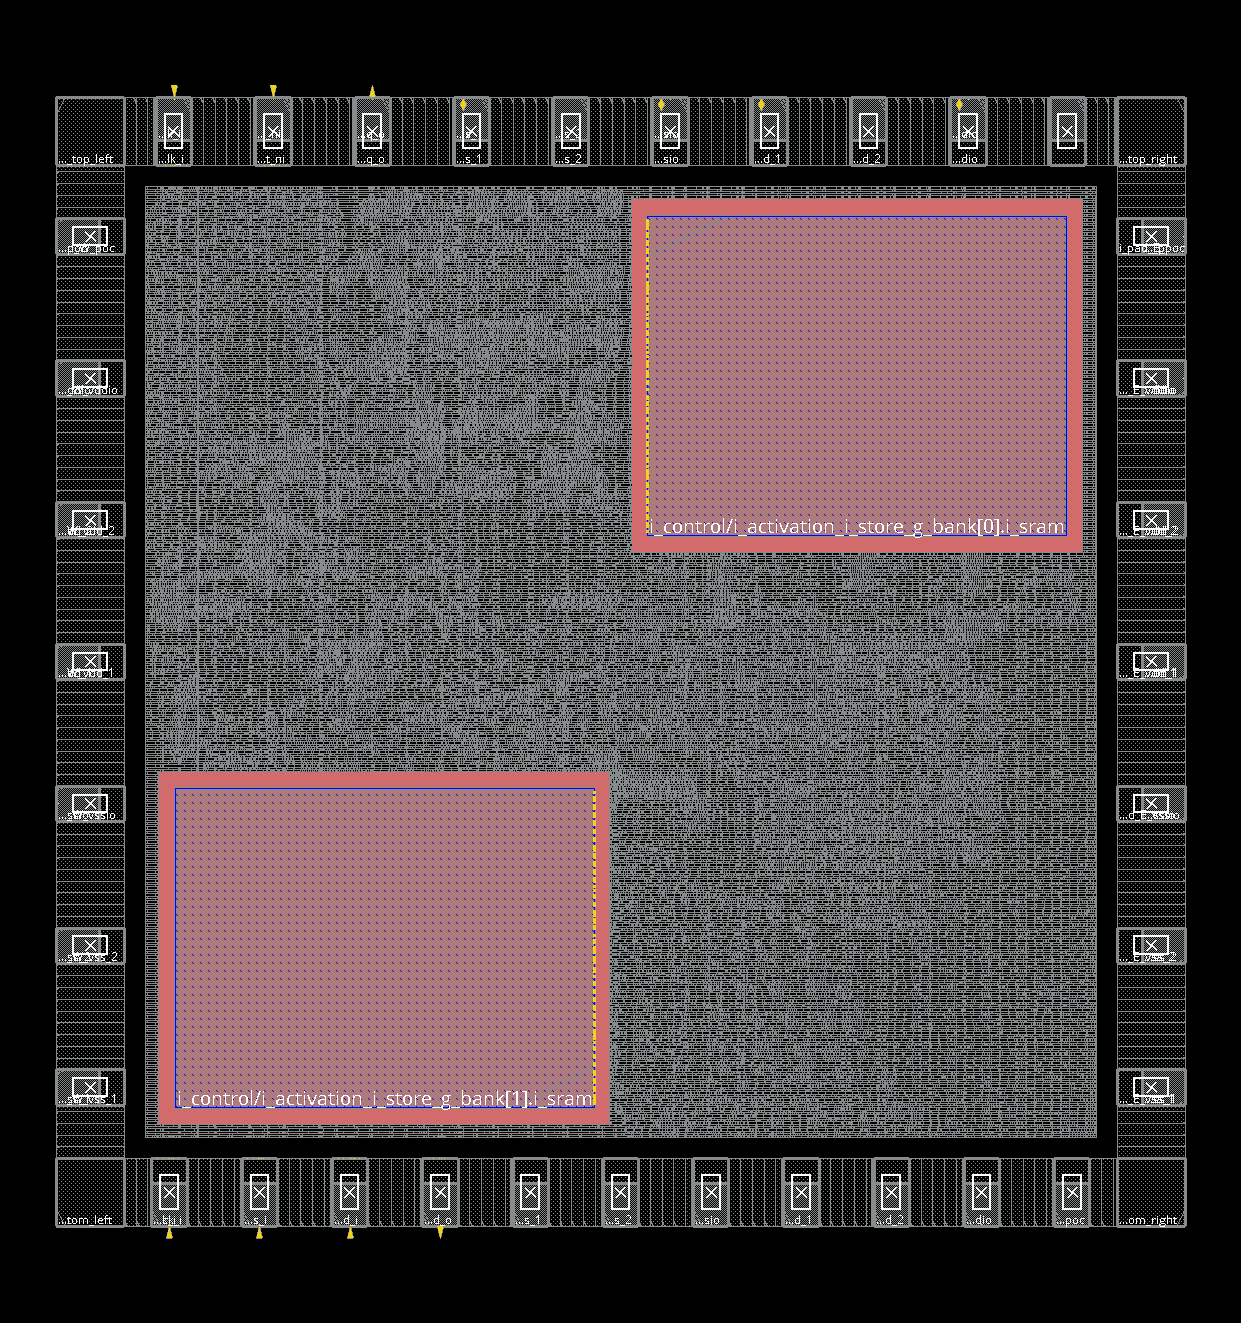
\includegraphics[width=0.225\linewidth]{figs/1_placement.png} &
    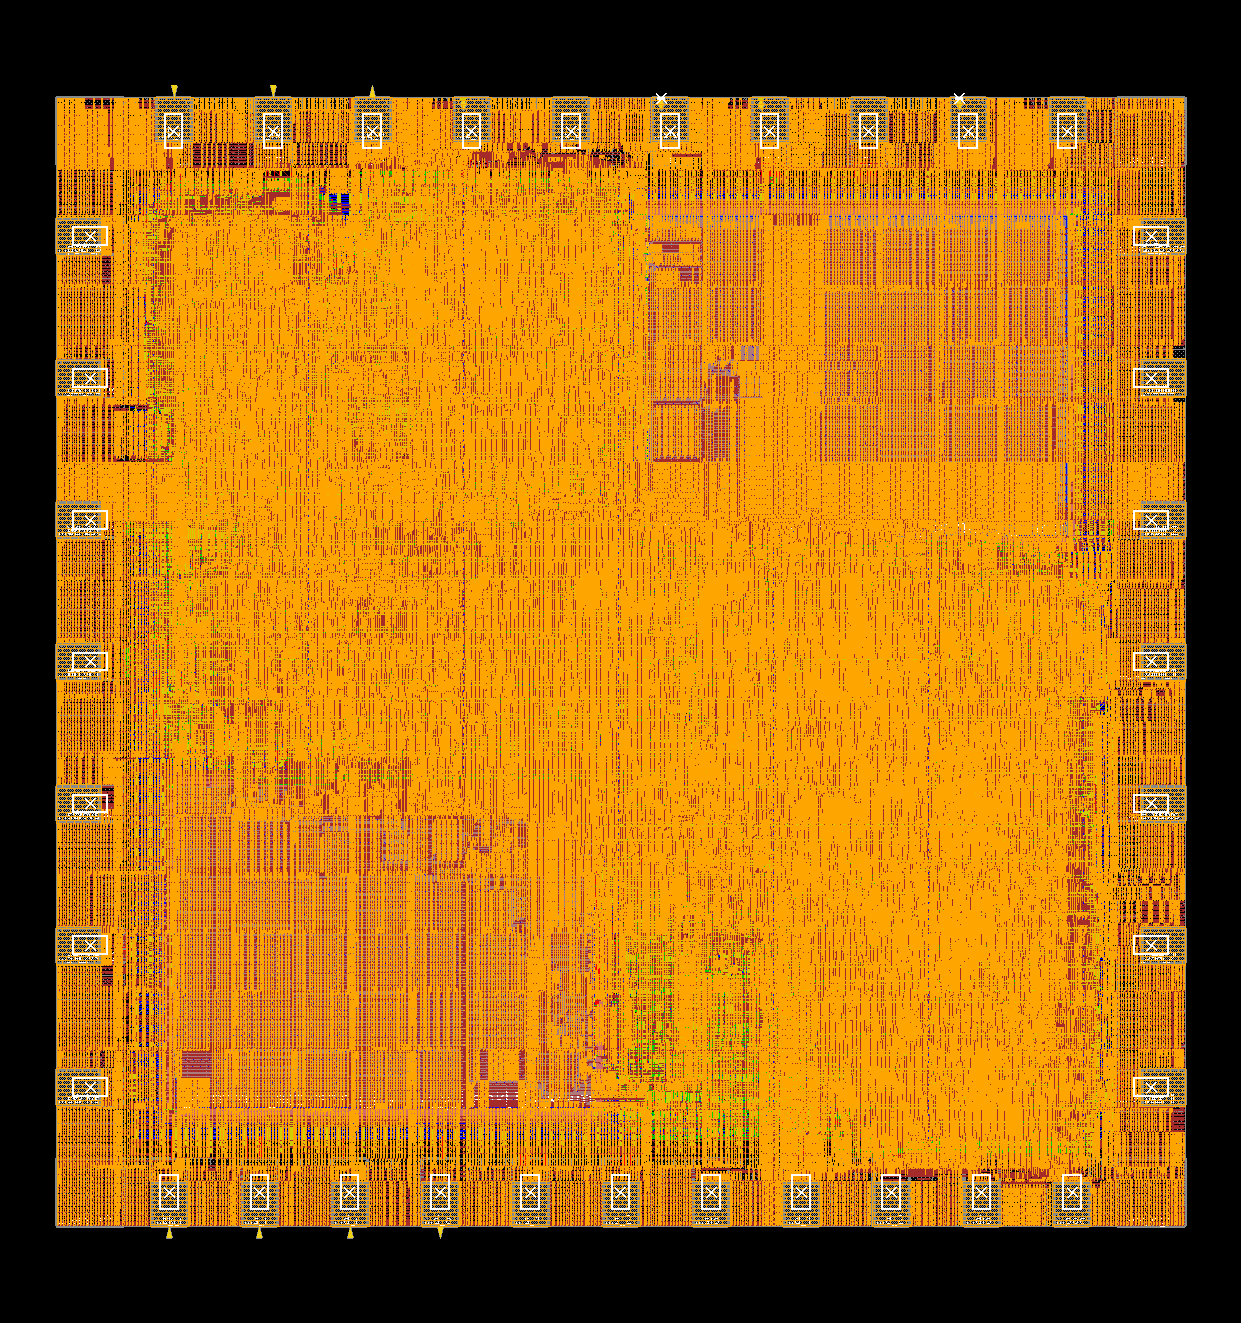
\includegraphics[width=0.225\linewidth]{figs/5_all.png} &
    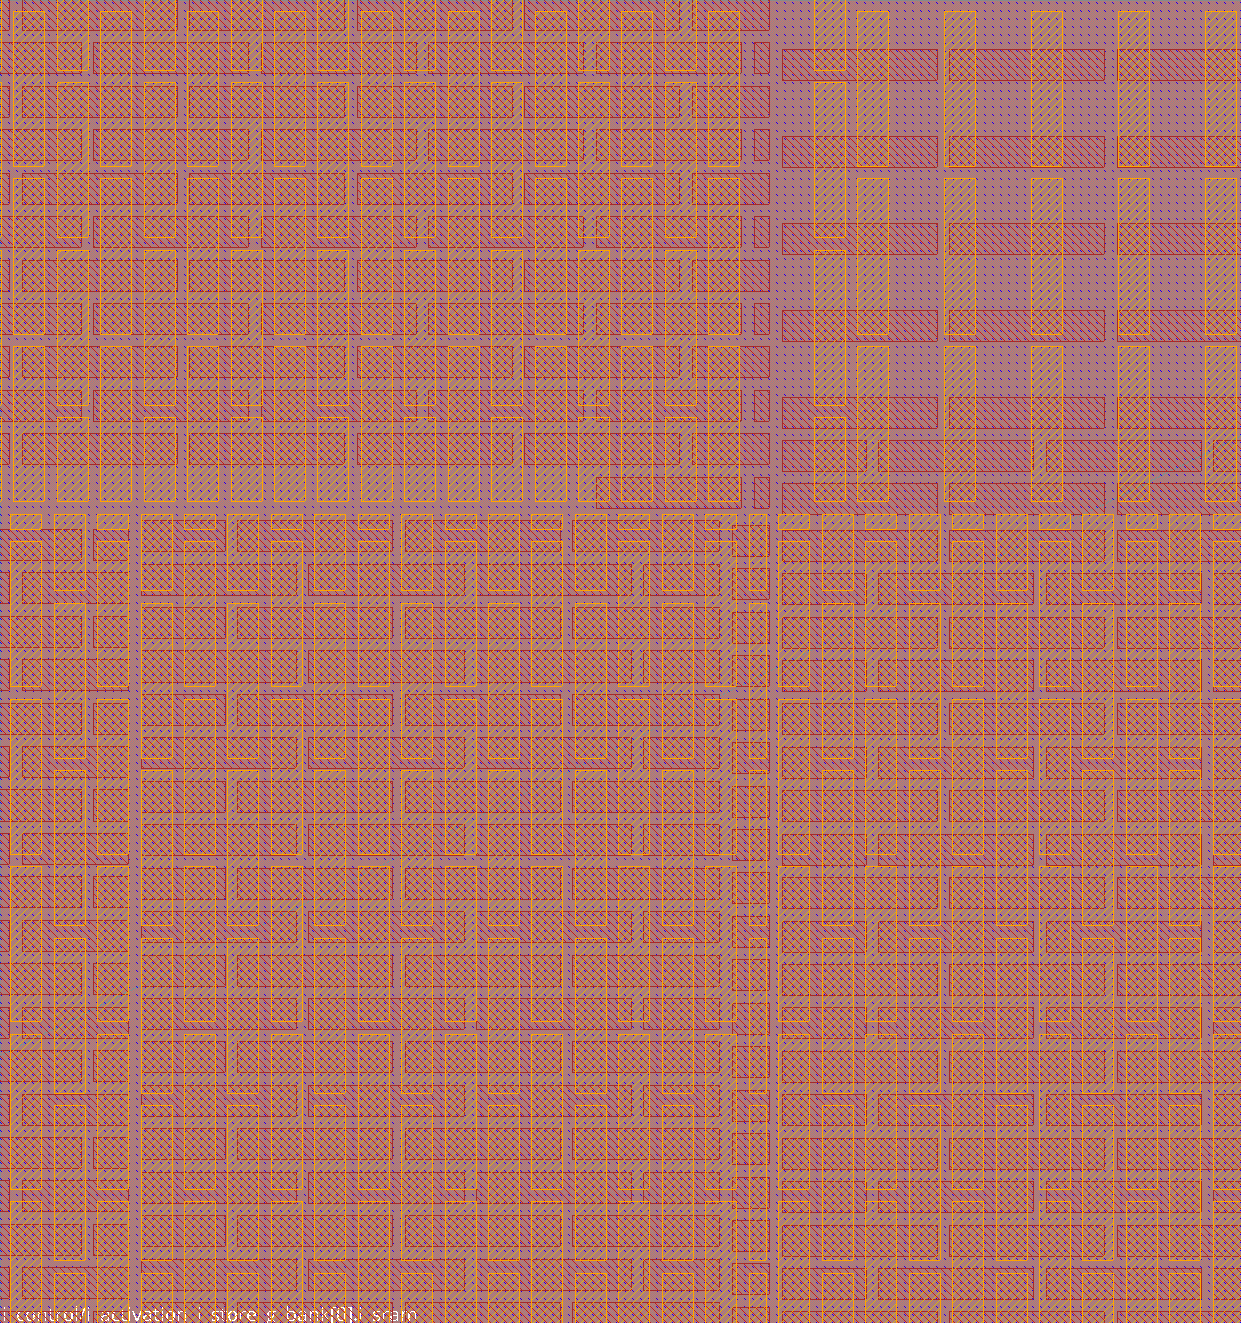
\includegraphics[width=0.225\linewidth]{figs/4b_m56_with_fill.png} &
    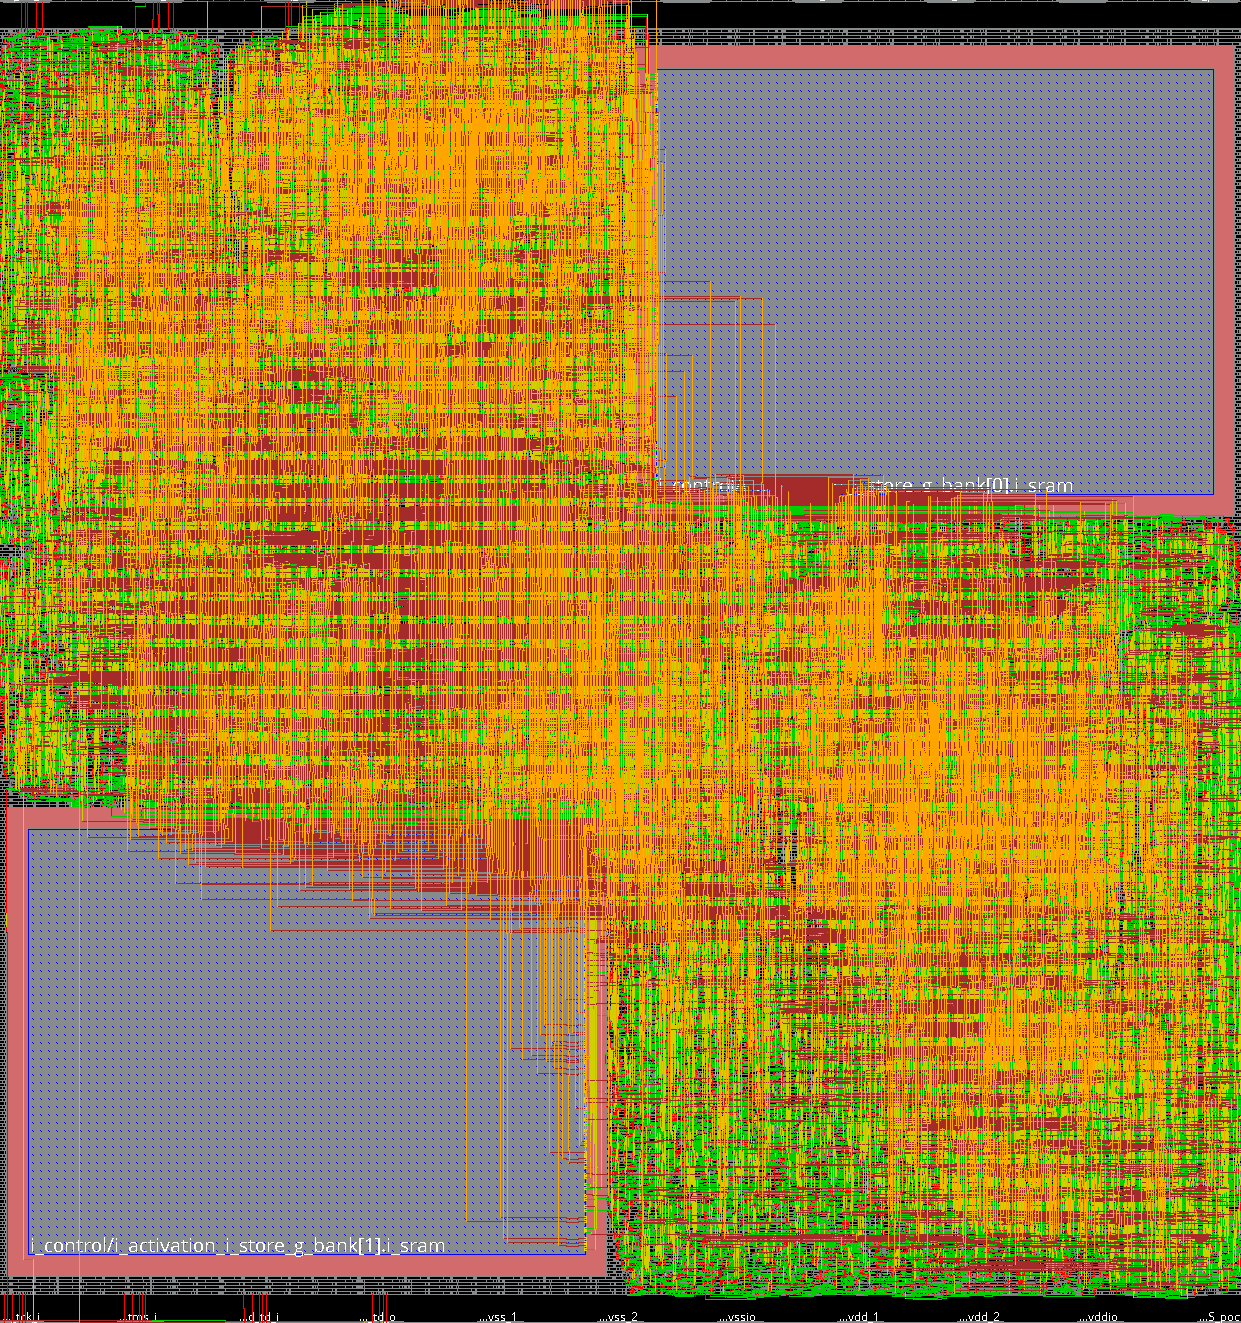
\includegraphics[width=0.225\linewidth]{figs/7_sram_diag_zoom.png} \\
    \scriptsize 对角双 SRAM 平面规划 & \scriptsize 全信号布线 M1–M6 & \scriptsize M5/M6 金属填充 & \scriptsize 对角 SRAM 间距通道
  \end{tabular}\par\vspace{10pt}
  \justifying
  \begin{columns}[T,onlytextwidth]
    \column{0.48\textwidth}
    \textbf{物理架构与 DRC 闭合}
    \begin{itemize}\setlength{\itemsep}{2pt}
      \item 未封环管芯 \hl{\NDieSide{} µm} ≤ \NDieLimit{} µm 预算（\NDieAfter{} mm²；\NMacroCount× \texttt{RA1SHD\_2048x32M8}，\NMacroArea{} mm²）
      \item Innovus 内部检查：\hl{\NGeoPass/\NGeoTotal} \NGeoStatus
      \item \NPadCount{} 个 \texttt{PAD60LU\_OBV} CUP Pad：布线前施加 \NPadMargin{} µm M5/M6 路由与填充 Keepout
    \end{itemize}
    \column{0.48\textwidth}
    \textbf{布线后时序、SDF 与等价性验证}
    \begin{itemize}\setlength{\itemsep}{2pt}
      \item 布局后 SDF 门级仿真：\hl{\NSdfStatus}（\NSdfCmds{} 条 JTAG 指令，\NSdfUnexpected{} 个非预期告警）
      \item Formality LEC（RTL vs. 布线网表）：\texttt{\NLecVerified}
      \item OpenSTA TT stdcell+IO：Setup \NStaSetup{} ns / Hold \NStaHold{} ns；CTS/repair +\NCtsRepairArea{} kµm²
    \end{itemize}
  \end{columns}
\end{frame}

\begin{frame}{\NMmmcCorners-Corner MMMC STA、SRAM 接口与 \NCdcRows-Path CDC 闭合}
  \begin{columns}[T,onlytextwidth]
    \column{0.48\textwidth}
    {\scriptsize\setlength{\tabcolsep}{3pt}
    \begin{tabular}{@{}llrrl@{}}
      \toprule
      \textbf{Corner} & \textbf{时钟} & \textbf{Setup} & \textbf{Hold} & \\ \midrule
      \texttt{tt25} & \NCoreMHz{} MHz & \NTTSetup & \NTTHoldW & \NTTBadge \\
      \texttt{ff0} & \NCoreMHz{} MHz & \NFFzSetup & \NFFzHoldW & \NFFzBadge \\
      \texttt{ffm40} & \NCoreMHz{} MHz & \NFFmSetup & \NFFmHoldW & \NFFmBadge \\
      \rowcolor{surf}\texttt{ss125} & \NCoreMHz{} MHz & \hl{\NSSSetup} & \NSSHoldW & \NSSBadge \\
      \rowcolor{surf}\texttt{SS125\_DERATED} & \NSSDPeriod{} ns / \NSSDFreq{} MHz & \textbf{\NSSDSetup} & \NSSDHoldW & \NSSDBadge \\ \bottomrule
    \end{tabular}}\par\vspace{3pt}
    \snote{\NMmmcCorners{} 个 PVT Corner 的最差负 Slack（WNS，单位 ns）。}\vspace{5pt}
    \begin{itemize}\setlength{\itemsep}{2pt}
      \item TT 与两个 FF corner 在 \NCoreMHz{} MHz 下\NCleanMmmcStatus（TNS = \NTTTns/\NFFzTns/\NFFmTns{} ns，最小 Hold \NCleanHoldMin{} ns @ \texttt{\NCleanHoldMinCorner}）。
      \item \texttt{ss125} 在 \NCoreMHz{} MHz 下 TNS = \NSSTns{} ns（\NSSViol{} 端点，关键路径止于 \NSSEndSram{} \texttt{WEN}，到达 \NSSArr{} vs. 要求 \NSSReq{} ns）；降频至 \NSSDFreq{} MHz 后\NSSDStatus。
    \end{itemize}\par\vspace{5pt}
    \callout[warnink]{\textbf{RC 范围说明}：\texttt{\NRcNote}。综合/P\&R 以 TT 为目标；通过 MMMC 优化闭合 \texttt{ss125} 是 Phase B 首要任务。}
    \column{0.49\textwidth}
    \textbf{SRAM 接口时序（\NSramRows{} 视图，ns）}\par\vspace{2pt}
    {\scriptsize\setlength{\tabcolsep}{2.5pt}
    \begin{tabular}{@{}llrrrr@{}}
      \toprule
      \textbf{Corner} & \textbf{角色} & \textbf{Setup→} & \textbf{Hold→} & \textbf{Setup←} & \textbf{Hold←} \\ \midrule
      \tabinput{data/sram_rows.tex}
      \bottomrule
    \end{tabular}}\par\vspace{7pt}
    \textbf{JTAG ↔ Core CDC 签核}
    \begin{itemize}\setlength{\itemsep}{2pt}
      \item \NCdcPaths{} 条路径 × \NCdcCorners{} corner = \hl{\NCdcPos/\NCdcRows{} 正 Slack}
      \item 最差 CDC 裕量：\NCdcMin{} ns @ \texttt{\NCdcMinCorner}
    \end{itemize}
  \end{columns}
\end{frame}

\begin{frame}{窗口化 \NPwAnnot\%-Annotated VCD 功耗与算子融合收益}
  \begin{columns}[T,onlytextwidth]
    \column{0.49\textwidth}
    \centering
    \begin{tikzpicture}
      \begin{axis}[issccbar, ybar, width=\linewidth, height=5.1cm, bar width=13pt, bar shift=0pt,
          ymin=0, ymax=70, ylabel={TT \NCoreMHz{} MHz 总功耗（mW）},
          xmin=-0.5, xmax=\NPowerXmax, xtick={0,...,\NPowerLast}, xticklabels/.expand once=\NPowerTicks,
          x tick label style={font=\tiny}, ymajorgrids,
          nodes near coords, nodes near coords style={font=\tiny, text=ink}]
        \input{data/power_plot.tex}
      \end{axis}
    \end{tikzpicture}\par\vspace{2pt}
    \snote{无向量参考（\NVlessRaw{} mW）高估真实 VCD 窗口 \NVlessOverMin–\NVlessOverMax×。}
    \column{0.48\textwidth}
    {\scriptsize
    \begin{tabular}{@{}lrrrr@{}}
      \toprule
      \textbf{工作负载} & \textbf{周期} & \textbf{窗口 µs} & \textbf{功耗 mW} & \textbf{能耗 µJ} \\ \midrule
      \tabinput{data/power_rows.tex}
      \bottomrule
    \end{tabular}}\par\vspace{10pt}
    \callout[peking]{\textbf{融合 vs. 非融合 CNN}：执行从 \NUnfusedCyc{} 周期降至 \NFusedCyc{} 周期（\hl{\NFusionSpeed× 加速}）；单次推理能耗从 \NUnfusedE{} 降至 \hl{\NFusedE{} µJ}（\hl{−\NFusionSave\%}）。}\par\vspace{8pt}
    \begin{itemize}\setlength{\itemsep}{2pt}
      \item 从 SDF 门级仿真严格在 \texttt{busy → irq} 窗口内提取；动态功耗（internal+switching）\NPwDynMin–\NPwDynMax{} mW，静态漏电 \NPwLeakDisp{} mW（≤ \NPwLeakMaxPct\%）。
      \item \NPwAnnot.0\% Toggle 标注覆盖全部 \NPwN{} 个工作负载（TT corner，典型 RC）。
    \end{itemize}
  \end{columns}
\end{frame}

\begin{frame}{物理收尾：Seal Ring、Dummy Fill 与 Keepout（\NDbuPerUm{} DBU/µm）}
  \centering
  % Crop the top Matplotlib title banner cleanly so figures keep crisp axes & legends only
  \begin{tabular}{@{}ccc@{}}
    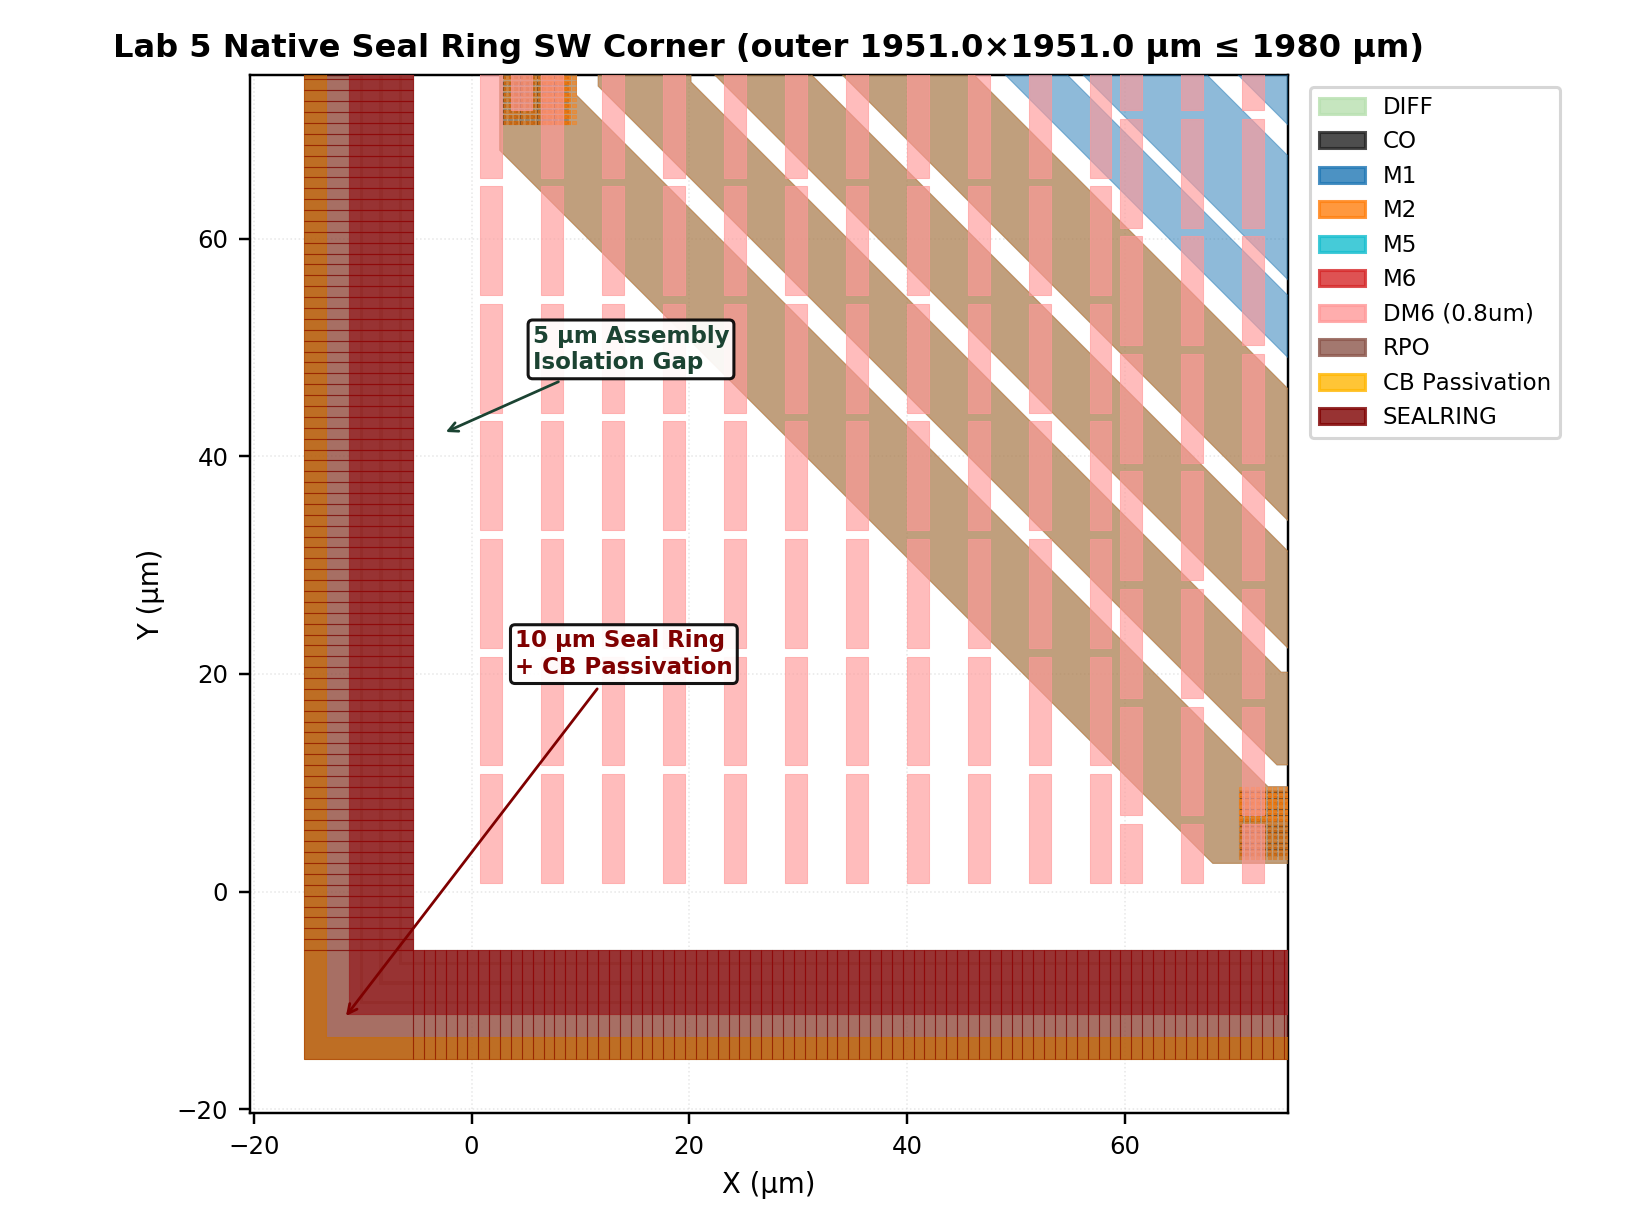
\includegraphics[width=0.312\linewidth, trim=0 0 0 22pt, clip]{figs/8_lab5_sealring_corner.png} &
    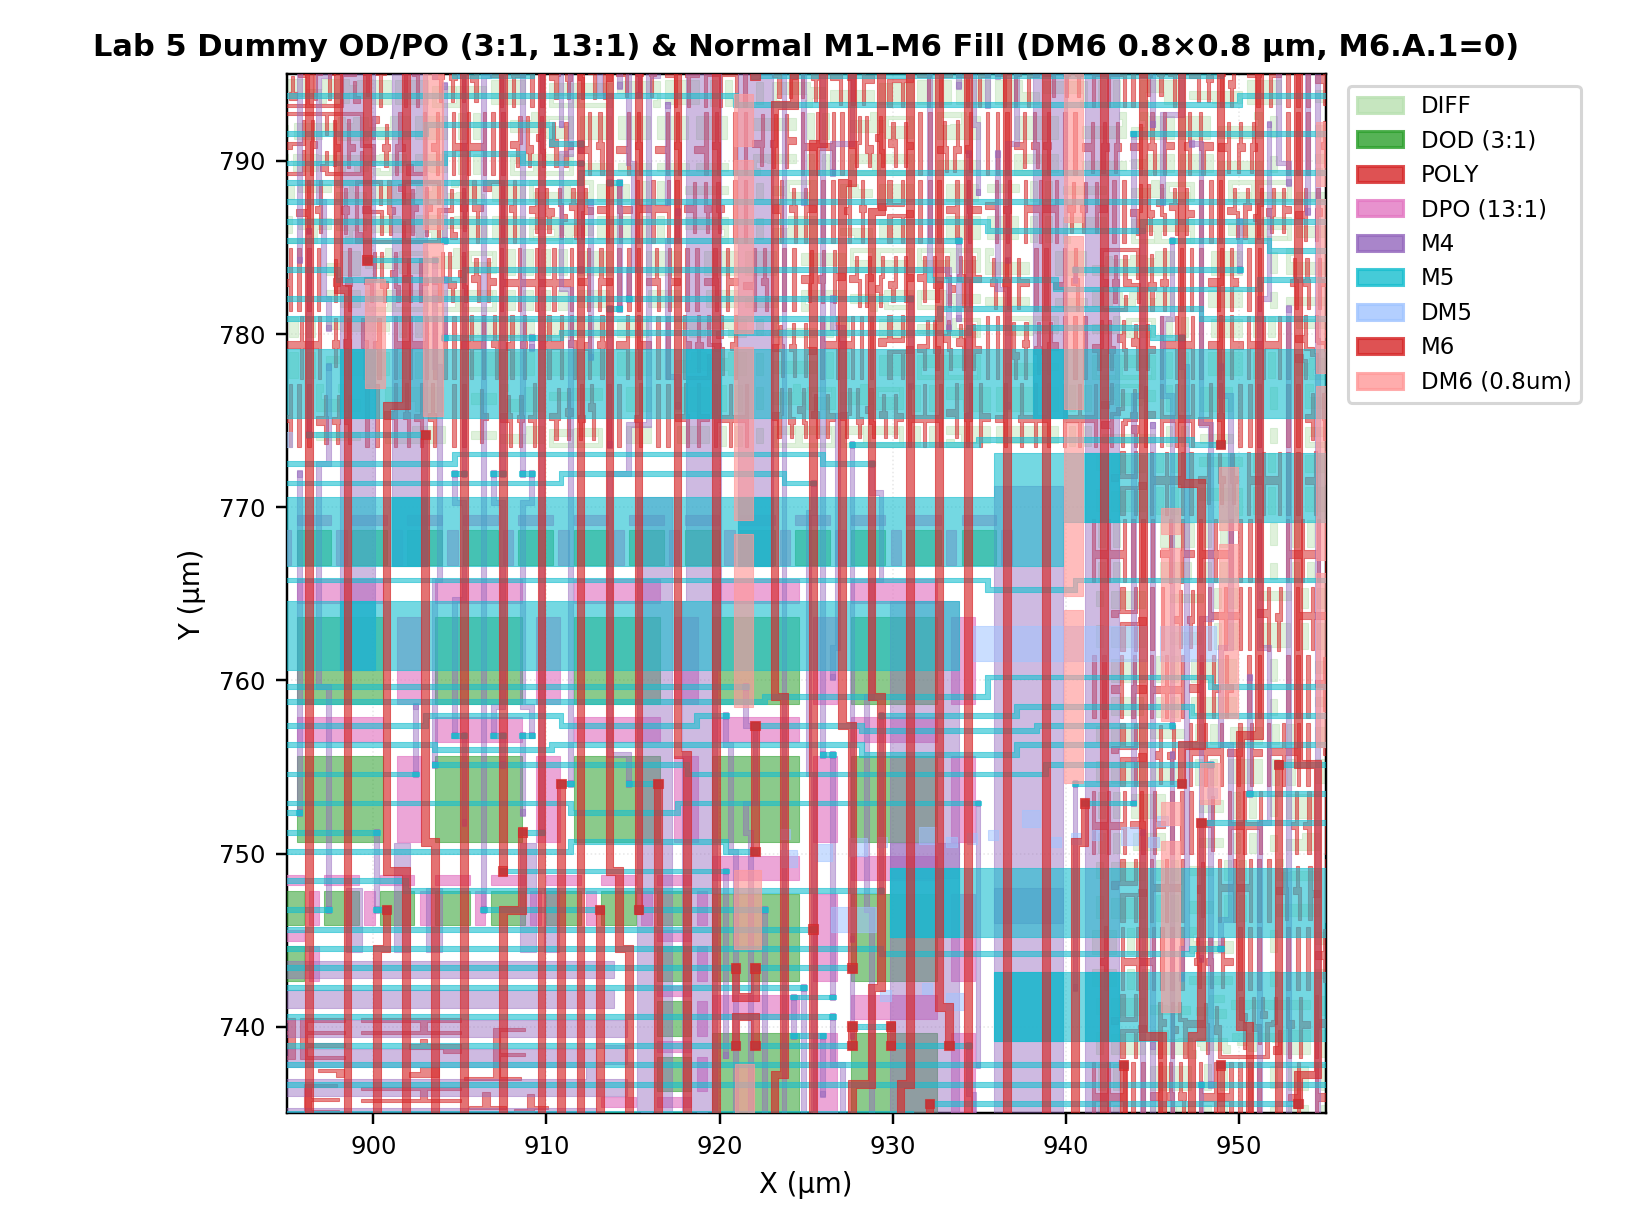
\includegraphics[width=0.312\linewidth, trim=0 0 0 22pt, clip]{figs/9_lab5_dummy_fill_zoom.png} &
    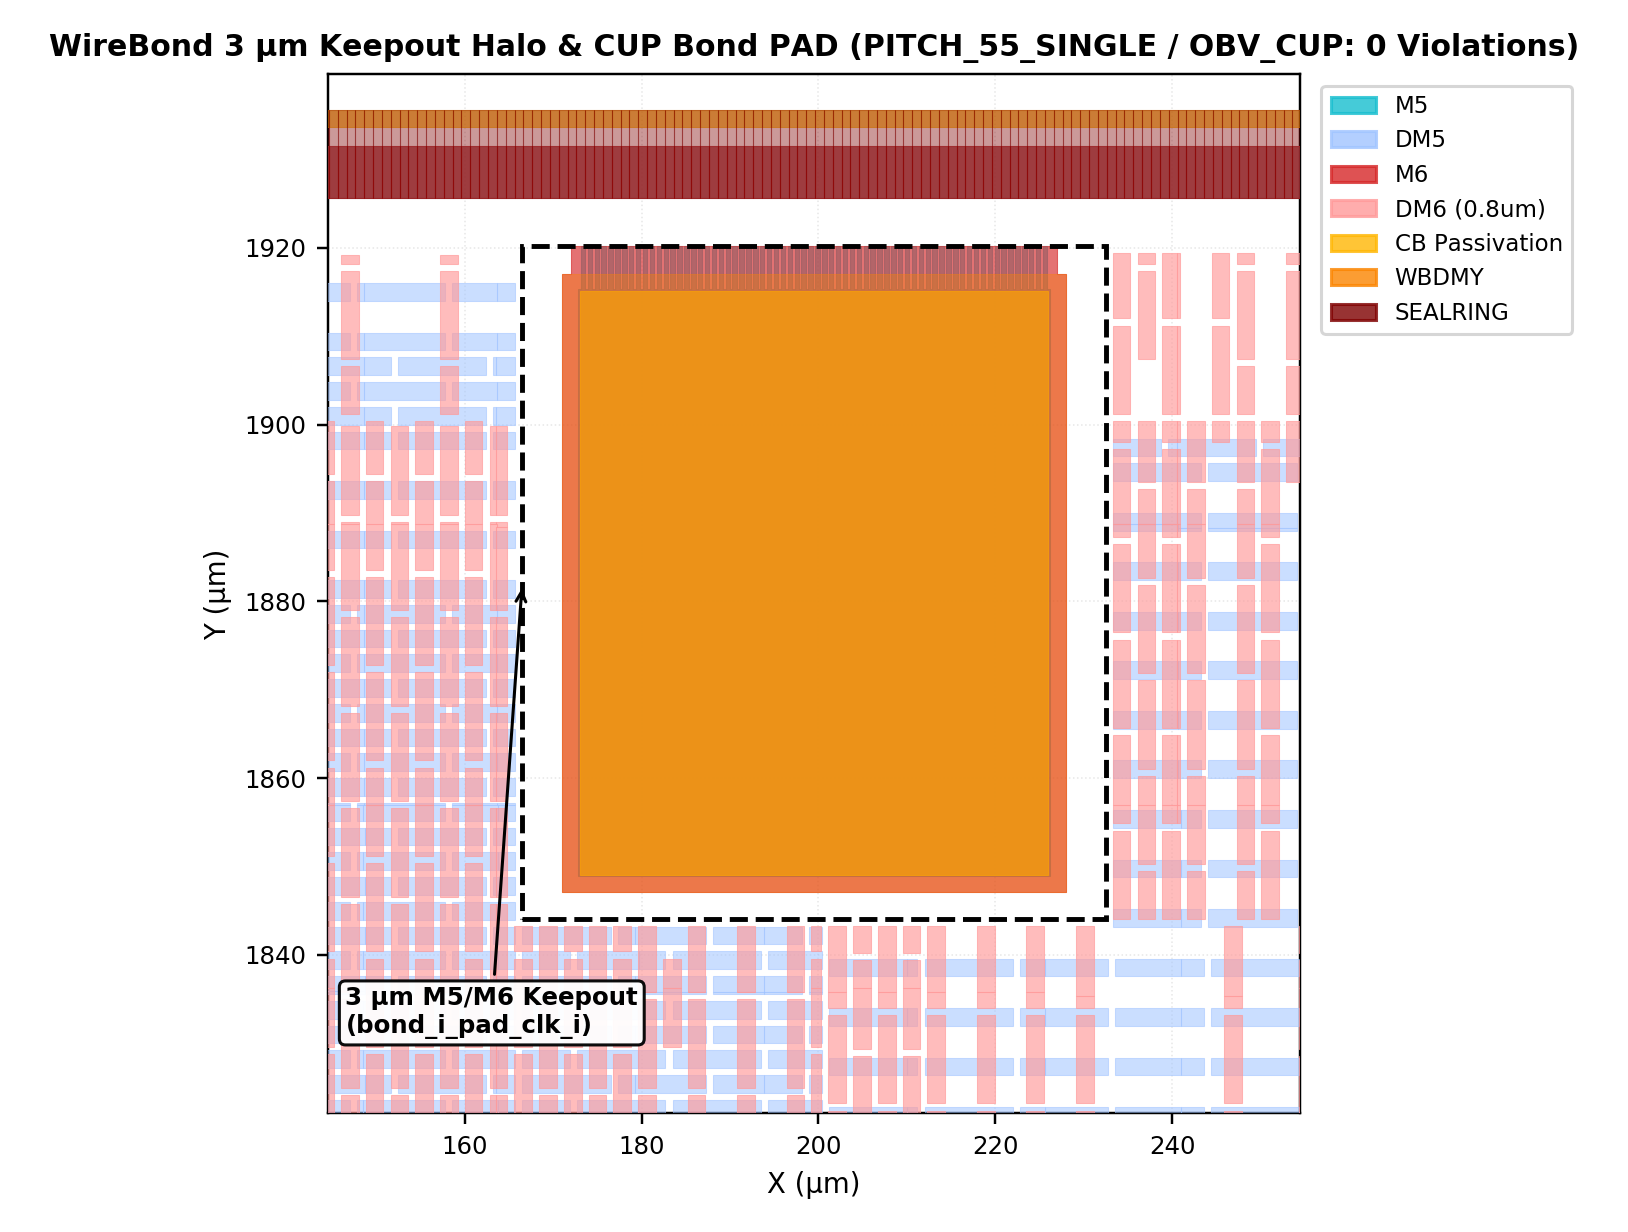
\includegraphics[width=0.312\linewidth, trim=0 0 0 22pt, clip]{figs/10_lab5_wirebond_keepout_zoom.png} \\[3pt]
    \scriptsize\textbf{原生 Seal Ring（西南角）} & \scriptsize\textbf{Dummy OD/PO + M1–M6 填充} & \scriptsize\textbf{WireBond Keepout 保护区}
  \end{tabular}\par\vspace{9pt}
  \justifying
  \begin{columns}[T,onlytextwidth]
    \column{0.315\textwidth}
    \scriptsize 原生 \NDbuPerUm{} DBU/µm Seal Ring 包围整数 µm 管芯框架：外部封环后管芯 \hl{\NSealSide×\NSealSide{} µm} ≤ \NSealLimit{} µm 预算。
    \column{0.315\textwidth}
    \scriptsize 全芯片 \texttt{Dummy\_OD\_PO}（\texttt{DOD}/\texttt{DPO}）+ \texttt{Dummy\_Metal} M1–M6；常规 M6 填充 \NDummyMsix×\NDummyMsix{} µm，M6.A.1 = \hl{\NDummyMsixViol}。
    \column{0.315\textwidth}
    \scriptsize 全部 \NPadCount{} 个 \texttt{PAD60LU\_OBV} 键合 Pad 保留 \NPadMargin{} µm M5/M6 路由与填充 Keepout（\NWbHier{} Hier. / \NWbExp{} Exp. Keepout/WireBond 违例）。
  \end{columns}
\end{frame}

\begin{frame}{全芯片物理签核矩阵与晶体管级 ERC 审计}
  \snote{所有验证引擎均在同一份 \NDbuPerUm{} DBU/µm \texttt{postDummy.gds}（\texttt{my\_soc\_top}，\NSealSide{} µm ≤ \NSealLimit{} µm）及 CDL 网表上执行。}\vspace{1pt}
  \begin{columns}[T,onlytextwidth]
    \column{0.52\textwidth}
    {\scriptsize
    \begin{tabularx}{\linewidth}{@{}l c >{\raggedright\arraybackslash}X@{}}
      \toprule
      \textbf{引擎} & \textbf{状态} & \textbf{已验证签核证据} \\ \midrule
      \textbf{DRC}+\texttt{CO.R.4} & \NDrcBadge & 未屏蔽 \NDrcRules{} 规则，阻断=\hl{\NDrcBlocking}；IO \texttt{CO.R.4} PIMP 修复 \NCorFourBefore{} → \hl{\NCorFourAfter} \\[1pt]
      \textbf{nmLVS} & \NLvsBadge & 全 SRAM 非黑盒，严格 \NLvsStrictTol\% 容差：\NLvsErr{} IO \texttt{R(PR)}（最大 \NLvsMax\%）；\NLvsTol\% 容差下 \hl{\texttt{\NLvsStatus}} \\[1pt]
      \textbf{Antenna} & \NAntBadge & \hl{\NAntHier{} Hier. / \NAntExp{} Exp.}，覆盖完整填充后管芯 \\[1pt]
      \textbf{WireBond} & \NWbBadge & \hl{\NWbHier{} Hier. / \NWbExp{} Exp.}，覆盖全部 \NWbRules{} 规则与 \NPadCount{} 个 \texttt{PAD60LU\_OBV} \\[1pt]
      \textbf{ERC} & 审计 & \NErcHier{} Hier. / \NErcExp{} Exp. 追溯至 vendor IO 子单元与外 Seal Ring \\ \bottomrule
    \end{tabularx}}\par\vspace{1pt}
    \centering\includegraphics[width=0.72\linewidth]{figs/11\_lab5\_cor4\_and\_erc\_audit.png}\par
    {\tiny\color{muted}左：\texttt{CO.R.4} PIMP 邻接修复；右：全芯片 ERC marker 分布。}
    \column{0.45\textwidth}
    {\scriptsize\setlength{\tabcolsep}{3pt}
    \begin{tabularx}{\linewidth}{@{}l r r >{\raggedright\arraybackslash}X@{}}
      \toprule
      \textbf{ERC 规则} & \textbf{Hier.} & \textbf{Exp.} & \textbf{晶体管/子单元核账} \\ \midrule
      \texttt{mnpg} & \NErcMnpgH & \NErcMnpgE & \NErcVddOneN×\NErcVddOneF{} \texttt{PVDD1CDG}+\NErcVddTwoN×\NErcVddTwoF{} \texttt{PVDD2CDG}+\NErcVddPocN×\NErcVddTwoF{} \texttt{PVDD2POC}：有源 rail ESD NMOS 箝位 \\[1pt]
      \texttt{nxwell\_float} & \NErcNxwellH & \NErcNxwellE & \multirow{2}{=}{\NErcVssN×\NErcVssD{} \texttt{PVSS1CDG}：\texttt{VSS}↔\texttt{VSSPST} 反并联 ESD 二极管阱/tap} \\
      \texttt{npvss49} & \NErcVssH & \NErcVssE & \\[1pt]
      \texttt{psub\_float} & \NErcPsubH & \NErcPsubE & \texttt{SR.S.1} 隔离带外侧 Seal Ring 衬底框架 \\ \bottomrule
    \end{tabularx}}\par\vspace{6pt}
    \callout[passink]{\textbf{审计结论}：\hl{\NErcDesignDefects{} 个设计/核心/SRAM ERC 缺陷}；Seal Ring 前后 ERC delta=\NErcPrePostDelta{}（\NErcPreH{}→\NErcHier{} Hier.，\NErcPreE{}→\NErcExp{} Exp.）；\texttt{SR.S.1} 隔离带未桥接。}\par\vspace{3pt}
    \callout[warnink]{\texttt{formal\_tapeout\_signoff=\NFormalTapeout}：vendor IO 与外框 ERC 条目保留，待 foundry 正式签核 waiver。}
  \end{columns}
\end{frame}


% ##################################################################### PART 03
\section{主机 JTAG 优化与 FPGA 验证}

\begin{frame}{EGo1 实板延迟分解：三步排除与双瓶颈归因}
  \callout[steel]{\textbf{三步排除}（EGo1 实板，\abi{} @ \NVivClk{} MHz，\texttt{\NVivPart}，\hl{\NFpgaTotal{} 次 \NFpgaExactStatus{} 推理}）：(1) NPU 实际计算仅 \hl{\NFpgaComputeMin–\NFpgaComputeMax{} ms}（≤ \NFpgaComputeMaxPct\% 驻留耗时，嵌在 \texttt{completion\_poll} 窗口内、未叠加在柱图中）；(2) \texttt{TCK} 1 → \NFpgaTckRatio{} MHz（\NFpgaTckRatio× 提频）零收益：\texttt{ecg} 驻留 \NFpgaEcgOneMs{} → \NFpgaEcgFiveMs{} ms，\texttt{gtsrb\_l} 输入 \NFpgaGtsrbInOneMs{} → \NFpgaGtsrbInFiveMs{} ms、模型上传 \NFpgaGtsrbUpOneMs{} → \NFpgaGtsrbUpFiveMs{} ms；(3) 冷启动模型上传占 \hl{\NFpgaUploadShare\%}（\NFpgaUploadMin–\NFpgaUploadMax{} ms）。}\par\vspace{2pt}
  \begin{columns}[T,onlytextwidth]
    \column{0.58\textwidth}
    \begin{tikzpicture}
      \begin{axis}[issccbar, xbar stacked, width=0.97\linewidth, height=3.9cm, bar width=10pt,
          xmin=0, xmax=330, xlabel={\NFpgaBestMhz{} MHz TCK 实测 EGo1 驻留推理耗时（ms）},
          symbolic y coords/.expand once=\NFpgaTicks, ytick=data, y dir=reverse,
          legend style={at={(0.5,1.03)}, anchor=south, legend columns=3, font=\tiny, draw=none, fill=none, /tikz/every even column/.append style={column sep=6pt}},
          xmajorgrids, enlarge y limits=0.14]
        \input{data/fpga_breakdown_plot.tex}
        \legend{固定控制/元数据 RPC, 分块数据 RPC, 主机包装残差}
      \end{axis}
    \end{tikzpicture}
    \column{0.39\textwidth}
    \textbf{\NFpgaBestMhz{} MHz TCK 耗时组成}\par\vspace{4pt}
    {\scriptsize
    \begin{itemize}\setlength{\itemsep}{3.5pt}
      \item \textbf{NPU 实际计算}：仅 \hl{\NFpgaComputeMin–\NFpgaComputeMax{} ms}（≤ \NFpgaComputeMaxPct\%，位于 poll 窗口内，不再叠加）。
      \item \textbf{固定控制/元数据 RPC}：几何均值 \hl{\NFpgaCtrlGeomean{} ms}（\NFpgaCtrlMin–\NFpgaCtrlMax{} ms）；主机包装残差 \NFpgaWrapMin–\NFpgaWrapMax{} ms。三段互斥，和严格等于驻留耗时。
      \item \textbf{分块数据读写}：\NFpgaXferMin–\NFpgaXferMax{} ms（几何均值 \NFpgaXferGeomean{} ms）；驻留总计 \NFpgaResMin–\NFpgaResMax{} ms（几何均值 \NFpgaRes{} ms）。
      \item \textbf{双瓶颈归因}：\texttt{ecg} 输入 \NFpgaEcgInWords{} word 与 \texttt{kws\_l} 输入 \NFpgaKwsLInWords{} word 同为 1 次 RPC，却耗时 \NFpgaEcgInRpcMs{} 与 \NFpgaKwsLInRpcMs{} ms；7 模型权重上传稳定在 \hl{\NFpgaUpMpwMin–\NFpgaUpMpwMax{} ms/word}（\texttt{gtsrb\_l} 输入 \NFpgaGtsrbInMpw{} ms/word）。耗时由主机 TCP RPC 往返与 OpenOCD 逐 \texttt{drscan} 同步 USB 刷新（\texttt{jtag\_execute\_queue()}）共同主导。
    \end{itemize}}
  \end{columns}
\end{frame}

\begin{frame}{Host JTAG Burst 与 Single-RPC 流水化：分层实测证据与边界}
  \noindent{\color{ink}\scriptsize
  \begin{tabular*}{\linewidth}{@{\extracolsep{\fill}}l r r r r r r@{}}
    \toprule
    & \multicolumn{2}{c}{\textbf{\NRtlTckMhz{} MHz TCK RTL Wire Sim}} & \multicolumn{4}{c}{\textbf{Live \texttt{TclRpc} TCP + \texttt{tclsh} OpenOCD-Protocol Sim}} \\
    \cmidrule(lr){2-3}\cmidrule(lr){4-7}
    \textbf{Model} & \textbf{Burst (ms)} & \textbf{上传 \%} & \textbf{Batched → Pipe RPC} & \textbf{RPC 减少} & \textbf{TCP+tclsh (ms)} & \textbf{× 加速} \\ \midrule
    \tabinput{data/jtag_sim_rows.tex}
    \bottomrule
  \end{tabular*}}\par\vspace{9pt}
  \begin{columns}[T,onlytextwidth]
    \column{0.48\textwidth}
    \textbf{分层实测：各层证明了什么}
    \begin{itemize}\setlength{\itemsep}{2pt}
      \item \textbf{\NRtlTckMhz{} MHz RTL 线层仿真}：证明 \texttt{IR 13h/14h} Burst 的物理线层下限为 \hl{\NRtlBurstMsMin–\NRtlBurstMsMax{} ms}（模型上传占 \NRtlUpPctMin–\NRtlUpPctMax\%）；\NRtlAnchorCount{} 个 \NRtlTckMhz{} MHz wordwise 锚点 \NRtlAnchorWordMin–\NRtlAnchorWordMax{} → \NRtlAnchorBurstMin–\NRtlAnchorBurstMax{} ms（提速 \NRtlAnchorSpMin–\NRtlAnchorSpMax×），与 \NRpcModels{} 模型 TCK 缩减 \NRtlTckCutMin–\NRtlTckCutMax× 一致。
      \item \textbf{Single-RPC 协议仿真}：\texttt{chipdesign\_reads/load/infer\_v5} 将 \NRpcBatchedMin–\NRpcBatchedMax{} 次 RPC（缓存清单 \NRpcCachedMin–\NRpcCachedMax{} 次）合并为 \hl{\NRpcPipe{} 次}（\NRpcPipeLoad{} load + \NRpcPipeInfer{} infer），往返减少 \hl{\NRpcSpMin–\NRpcSpMax×}。
    \end{itemize}
    \column{0.48\textwidth}
    \textbf{Loopback 执行、诚实边界与剩余瓶颈}
    \begin{itemize}\setlength{\itemsep}{2pt}
      \item \textbf{本地 TCP + \texttt{tclsh} 仿真}（golden-output SRAM fixture，计算正确性已由 RTL 仿真独立验证）：\hl{\NRpcExactCount/\NRpcModels{}} \NRpcExactStatus，loopback 中位数 \NRpcTcpBatchedMin–\NRpcTcpBatchedMax{} → \hl{\NRpcTcpPipeMin–\NRpcTcpPipeMax{} ms}。\textbf{不含真实 USB/FT232H 延迟，不等同于实板墙钟加速比。}
      \item \textbf{剩余瓶颈}：Single-RPC 未减少 \texttt{drscan} 总次数（仍为 \hl{\NRpcDrscanMin–\NRpcDrscanMax{} 次}）；若 OpenOCD 仍逐 \texttt{drscan} 同步刷新 USB，大头延迟仍在。
      \item \textbf{Phase B}：纯主机侧 \texttt{pyftdi} MPSSE 批量 USB 后端（打包为 1–5 个 USB Bulk 包）或 OpenOCD \texttt{svf} 批处理；EGo1 实板复测 SRAM-lookup + Single-RPC。
    \end{itemize}
  \end{columns}
\end{frame}

% ##################################################################### PART 04
\section{六场景应用与下一阶段计划}

\begin{frame}{六场景统一应用软件与验证}
  \noindent{\scriptsize
  \begin{tabularx}{\linewidth}{@{}l >{\raggedright\arraybackslash}X >{\raggedright\arraybackslash}X@{}}
    \toprule
    \textbf{场景} & \textbf{输入与处理流程} & \textbf{待完成硬件/现场项} \\ \midrule
    ECG 心跳分类 & MIT-BIH 心拍回放，5 分类 & 实时模拟前端 / MAX30102 传感器 \\
    HAR 活动识别 & UCI HAR 回放或实时手机 IMU CSV 流 & 佩戴式姿态标定 / MPU6050 \\
    MNIST 数字 & 交互画布（松笔触发） & 手写参与者评测集 \\
    KWS 语音 & 实时麦克风 + MFCC 前端，4 目标关键词 & 室内噪声物理麦克风验收 \\
    表情识别 & 最大人脸裁剪 → INT4 7 类 CNN & 准确率基线；实地测试 \\
    人脸检测 & CPU YuNet 默认 + 可选 NPU INT4 检测器 & NPU 检测器 QAT 精度调优 \\ \bottomrule
  \end{tabularx}}\par\vspace{10pt}
  \begin{columns}[T,onlytextwidth]
    \column{0.33\textwidth}
    \textbf{软件参考闭合}\par\vspace{2pt}
    \begin{itemize}\setlength{\itemsep}{2pt}
      \item 固定输入 \hl{\NDemoGolden/\NDemoGoldenTotal}：INT32 全输出 \NDemoExactStatus
      \item zoo 参考 \NDemoZoo/\NDemoZoo{} 帧 \NDemoExactStatus
      \item \NDemoUnit{} 个演示 + \NDemoJtag{} 个 JTAG 单元测试\NDemoUnitStatus
    \end{itemize}
    \column{0.33\textwidth}
    \textbf{\NDemoFixes{} 项运行时健壮性修复}\par\vspace{2pt}
    \begin{itemize}\setlength{\itemsep}{2pt}
      \item 浏览器重启等待上传队列清空
      \item HAR 流式窗口在 > \NHarGapMs{} ms 间隙后干净重置
      \item 自测严格区分局部与全量覆盖
    \end{itemize}
    \column{0.31\textwidth}
    \textbf{视觉模型基线}\par\vspace{2pt}
    \begin{itemize}\setlength{\itemsep}{2pt}
      \item 表情：\NEmoAcc\%（FER2013 \NEmoSamples{} 样本）
      \item 人脸 P/R/F1：\NFaceP/\NFaceR/\NFaceF\%
      \item \texttt{fpga\_validated=\NDemoFpga}（待上板）
    \end{itemize}
  \end{columns}
\end{frame}

\begin{frame}{诚实边界与 Phase B 工程计划}
  \begin{columns}[T,onlytextwidth]
    \column{0.48\textwidth}
    \textbf{\color{ink}已验证基线}\par\vspace{4pt}
    {\scriptsize
    \begin{tabularx}{\linewidth}{@{}l >{\raggedright\arraybackslash}X@{}}
      \toprule
      \textbf{RTL} & SRAM 化 \texttt{npu\_tensor\_lookup}：面积 \NLookupAreaPct\%，\NMutKilled/\NMutNew{} mutant，\NRtlModels{} 模型 \NRtlExactShort \\[3pt]
      \textbf{ASIC} & 统一 Single-GDS 流程：\NCoreMHz{} MHz TT/FF \NCleanMmmcStatus，SDF \NSdfStatus，LEC \texttt{\NLecVerified}，\NPwAnnot\%-VCD 功耗（算子融合节能 \NFusionSave\%） \\[3pt]
      \textbf{签核} & \NDbuPerUm{} DBU/µm \texttt{postDummy.gds}（\NSealSide{} µm）：DRC / 全 SRAM LVS / ANT / WireBond \NSignoffAllStatus，ERC 审计 \\[3pt]
      \textbf{主机} & \NRtlTckMhz{} MHz RTL + TCP/\texttt{tclsh} Single-RPC 仿真（\NRpcBatchedMin–\NRpcBatchedMax{} → \NRpcPipe{} RPC；\NRpcExactCount/\NRpcModels{} golden-output fixture \NRpcExactStatus） \\[3pt]
      \textbf{演示} & 六场景主机套件：\NDemoGolden/\NDemoGoldenTotal{} \NDemoExactStatus，\NDemoZoo/\NDemoZoo{} zoo 帧 \\ \bottomrule
    \end{tabularx}}
    \column{0.48\textwidth}
    \textbf{\color{peking}Phase B 工程计划与开放签核项}\par\vspace{4pt}
    {\scriptsize
    \begin{tabularx}{\linewidth}{@{}l >{\raggedright\arraybackslash}X@{}}
      \toprule
      \textbf{MMMC} & 服务器端真 MMMC：\texttt{ss125} setup + \texttt{ffm40} hold 联合优化；若纯后端 < 45 MHz，自动插 1 级 RTL 流水线（\texttt{i\_npu → i\_activation\_i\_store → i\_sram/WEN}），全量复跑回归 + Single-GDS 签核 \\[3pt]
      \textbf{签核} & Post-dummy RC/静态 IR 敏感度分析；获取 foundry ERC waiver（\texttt{formal\_tapeout\_signoff=\NFormalTapeout}） \\[3pt]
      \textbf{FPGA} & Vivado 实机指导包：Step 1 实板测 Single-RPC + OpenOCD，分离 TCP 与 USB 占比；Step 2 实测 \texttt{pyftdi} MPSSE 批量 USB 后端（\texttt{0403:6014}）与 OpenOCD \texttt{svf}，同步完成六场景上板验证；现有 Single-RPC 结论仅限 golden-output fixture \\[3pt]
      \textbf{现场} & MAX30102、MPU6050、摄像头、麦克风端到端传感器评测；最终冻结发布 \\ \bottomrule
    \end{tabularx}}
  \end{columns}
  \par\vspace{8pt}
  \begin{center}
    
\includegraphics[width=0.14\linewidth]{Figures/PKU-emblem-names.png}\\[6pt]
    {\large\bfseries\color{peking} 谢谢}\quad{\color{muted}·}\quad{\large\color{muted} 欢迎提问与讨论}
  \end{center}
\end{frame}

\end{document}
